\documentclass{article}
\usepackage{graphicx}
\begin{document}

\author{Andrew Bartnof}
\title{Difference-in-Difference for GGRF}
\date{\today}
\maketitle

\section{Introduction}

This paper documents two difference-in-difference studies for the GGRF insurance project.
Both attempt to quantify the impact of a green energy project on a neighborhood's home appreciation rates.
Study 1 uses a traditional two-way fixed effect difference-in-difference schema.
Study 2 uses a multi-level linear regression model to model the same phenomenon in a more statistically robust way.

\section{Background}

If green energy projects (eg solar farms and wind turbines) are built near residential areas, these projects may hurt home values.
This gives home-owners an incentive to resist green projects in their neighborhoods, even if they support green projects in general.

We want to quantify this change in home values, so that we can help to develop a new kind of financial project; a parametric risk insurance payout for home-owners near green energy projects.
The idea is that for a limited around of time while the projects are being built, local home prices may be artificially lower than a home in a similar neighborhood with no green energy projects.
If the home owner decides to sell their property during this period, the insurance product could cover the difference between the real house value and the counterfactual house value.

In this paper, we will refer to these scenarios as \textbf{control} when there is no green construction happening in a neighborhood, and \textbf{manipulation}, when there is a green construction happening in a neighborhood.

\section{Data}

We'll use three key datasets:

\subsection{Zillow Home Prices}
This dataset lists the home prices for 26,344 zip-codes, between the years 2000 and 2024.
(It was collected before I jumped on the GGRF project so I can't give much more insight into it.)

\subsection{Large-Scale Solar Photovoltaic Sites}
The solar dataset\footnote{Fujita, K.S., Ancona, Z.H., Kramer, L.A. et al. Georectified polygon database of ground-mounted large-scale solar photovoltaic sites in the United States. Sci Data 10, 760 (2023). https://doi.org/10.1038/s41597-023-02644-8} lists thousands of large-scale solar photovoltaic sites.
For each known solar site, we extract both location and year of operation.
Note that Ben Hoen is an author of both this dataset and the turbine dataset.

\subsection{Wind Turbines}
This dataset\footnote{
Rand, J.T., Kramer, L.A., Garrity, C.P. et al. A continuously updated, geospatially rectified database of utility-scale wind turbines in the United States. Sci Data 7, 15 (2020). https://doi.org/10.1038/s41597-020-0353-6} lists thousands of wind turbines.
Likewise, here, for each site, we extract both location and year of operation.

\subsection{Data Notes}
The Zillow home prices dataset only gives us zip-codes of homes.
As a result, we have linked each solar or turbine site to the zip-code that it most likely operates in.
We consider a neighborhood to be impacted (manipulated) by green construction if it shares a zip-code with one of these projects.
This is obviously a pretty rough spatial granularity, but it'll do.
We also round all dates in these three datasets to the nearest year.
Again, this is a rough temporal granularity, but again, it'll do.

\section{Study 1}

How did the rate of change of home appreciation change for zip-codes that had solar or turbine projects in them?

I think this study is really easy to understand with an example.
In 1979, Jimmy Carter put solar panels on his house, in zip-code 20500.
If we wanted to see if this solar panel project impacted the rate of home appreciation in zip-code 20500, we'd do the following:
Look at the year-over-year rate of home appreciation in 20500 in 1979, and for reference, include the previous few years (say, 1974-1979), and a few years after (say, 1979-1984).
Let's define home appreciation here as:

\noindent\textit{(current home price - last year's home price) / (last year's home price). }

Then we'd compare this to the median year-over-year rate of home appreciation of homes across the USA in zip-codes that didn't have any solar panels installed.
We'd see two trend lines-- that of our manipulation (zip-code 20500), and that of our control (all the other zip-codes without solar panels).

The problem with the above study is that our manipulation group has an n of 1, so it would be a good idea to expand our manipulation group to all other zip-codes in the USA that had solar panels installed in 1979.

This is the nature of study 1.
The results can be seen in figure \ref{study1solarfacets}.
\begin{figure}[h]
\centering
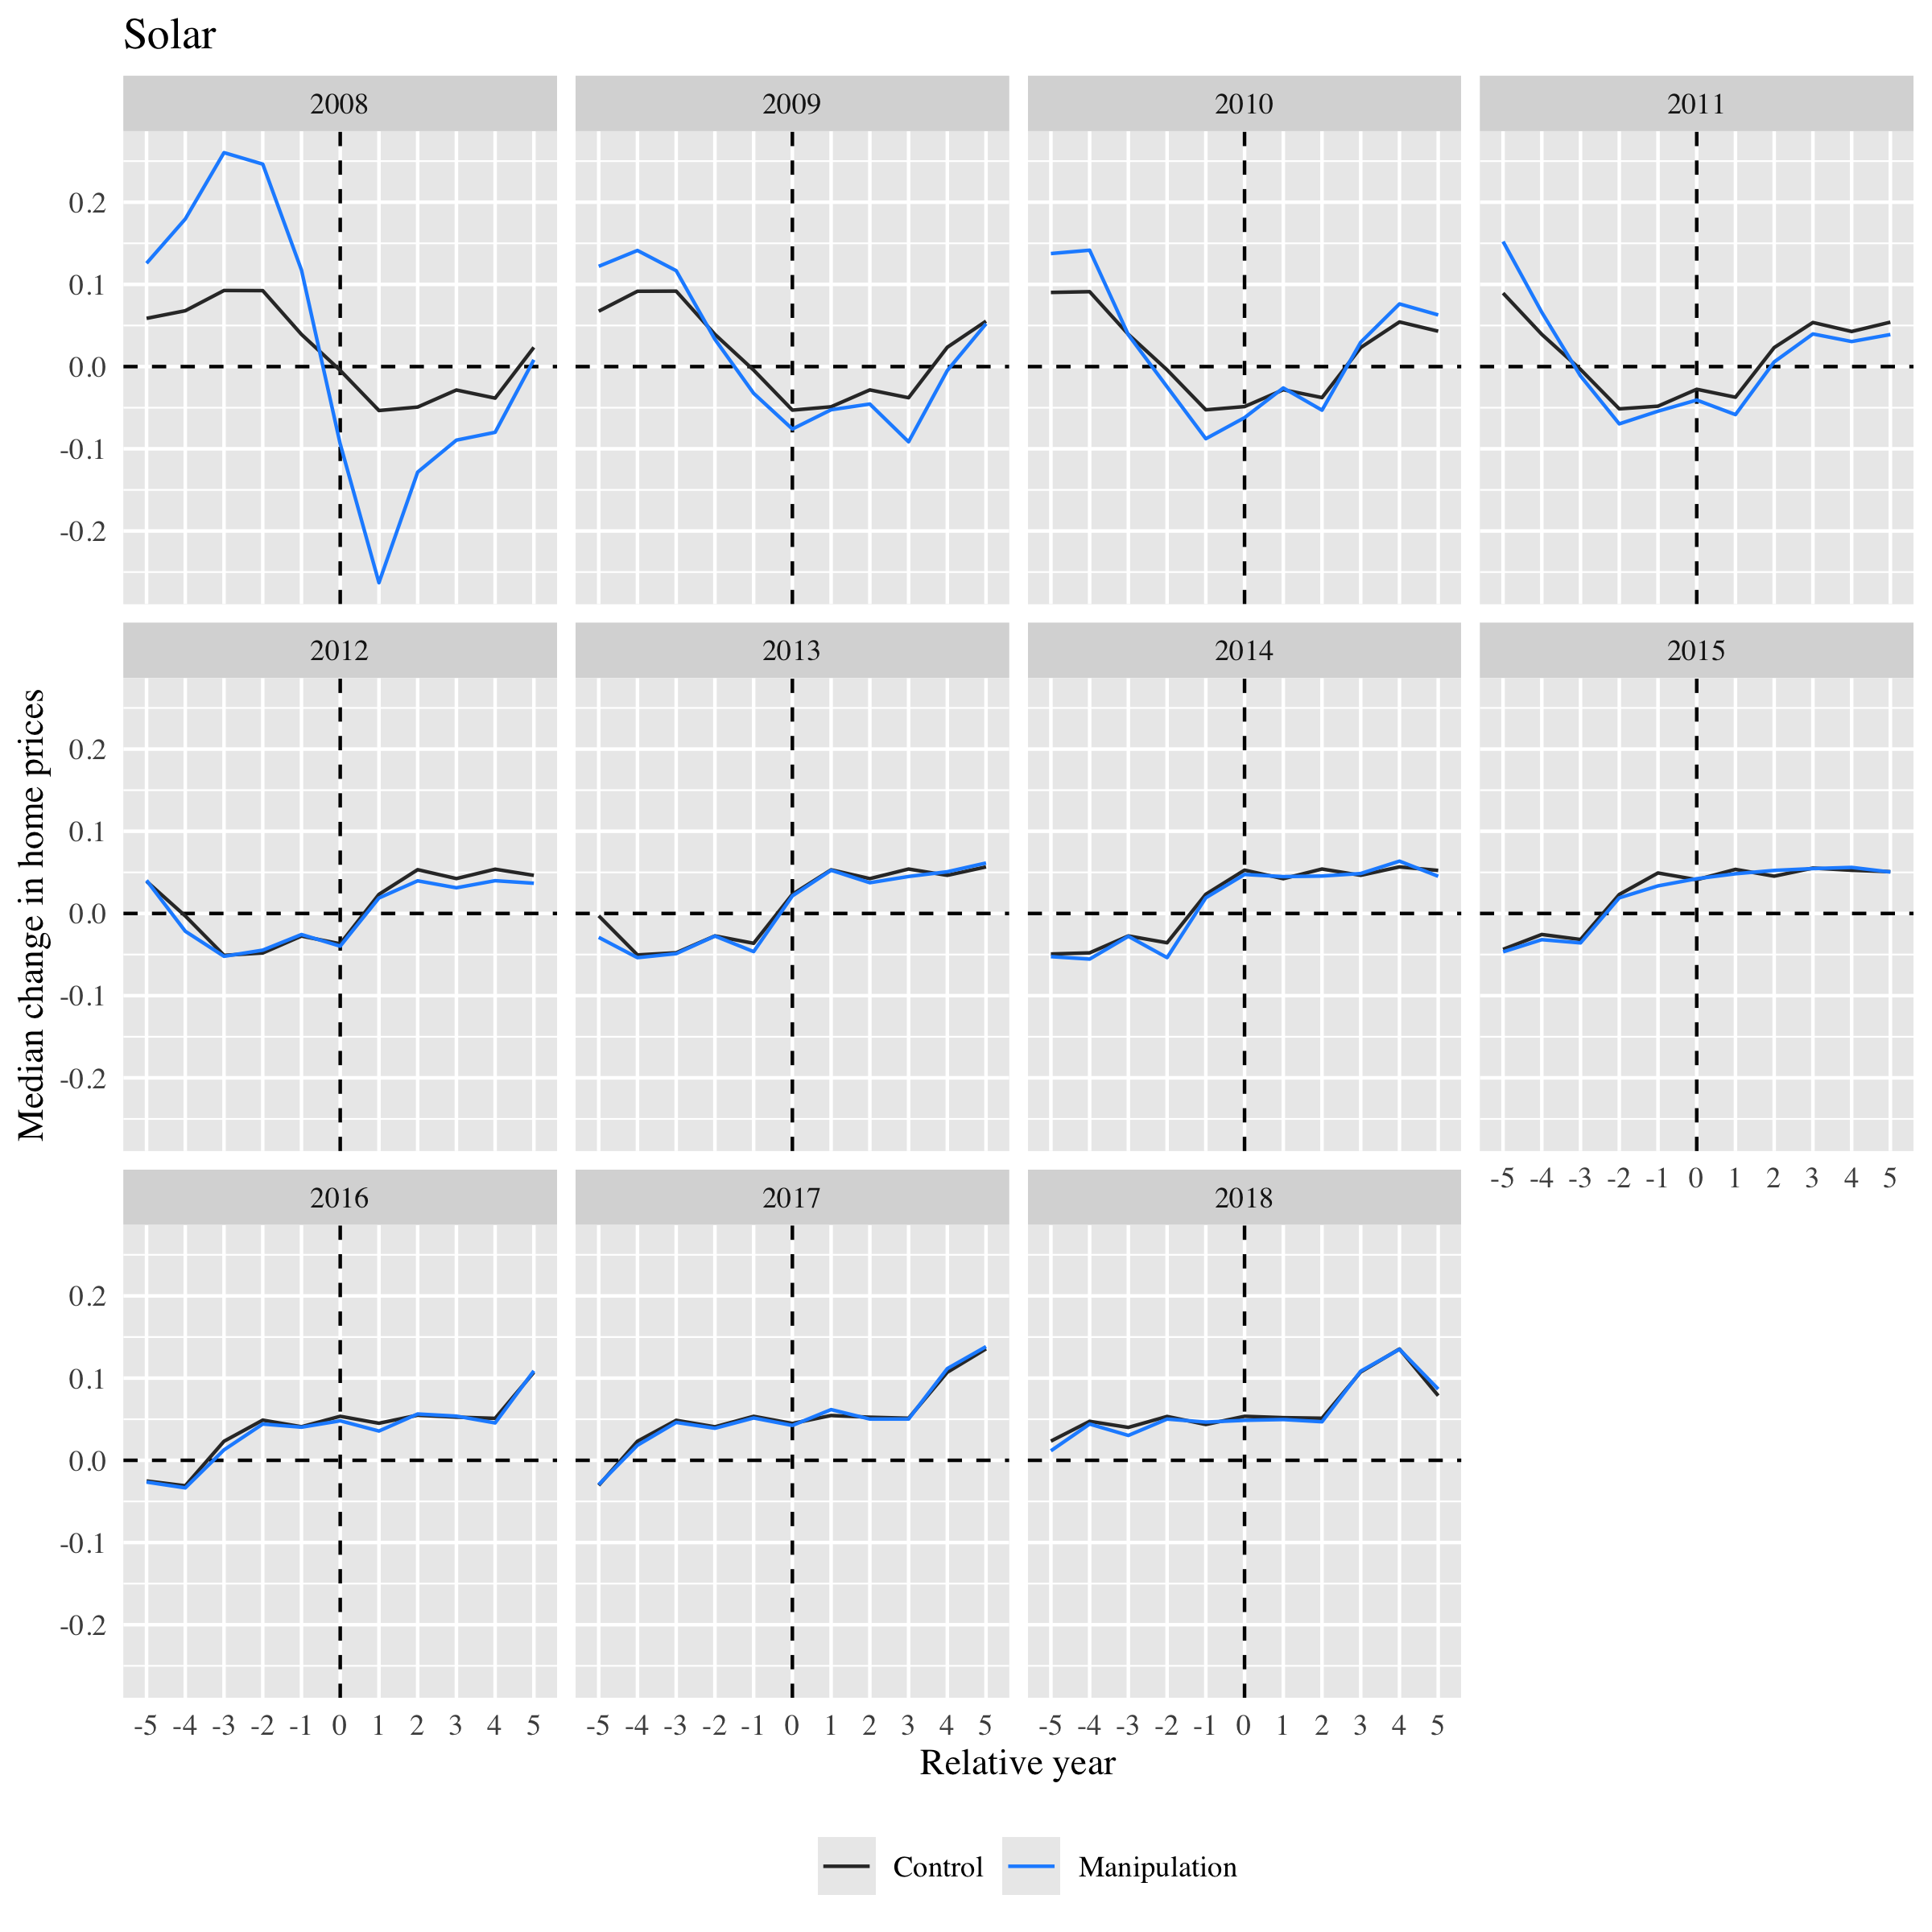
\includegraphics[width=0.9\linewidth]
{study1_solar_facets.png} 
\caption{Median change in home prices in zip-codes that had solar panels installed}
\label{study1solarfacets}
\end{figure}

Figure \ref{study1solarfacets} provides no useful insight, because it doesn't account for general changes in the real estate market.
For example, we can see the market tanking in 2008, but this completely confounds our ability to compare these lines to those a decade later.

Figure\ref{study1turbinefacets} shows us the DiD for turbine facilities, but it suffers from the same shortcomings as figure\ref{study1solarfacets}.
\begin{figure}[h]
\centering
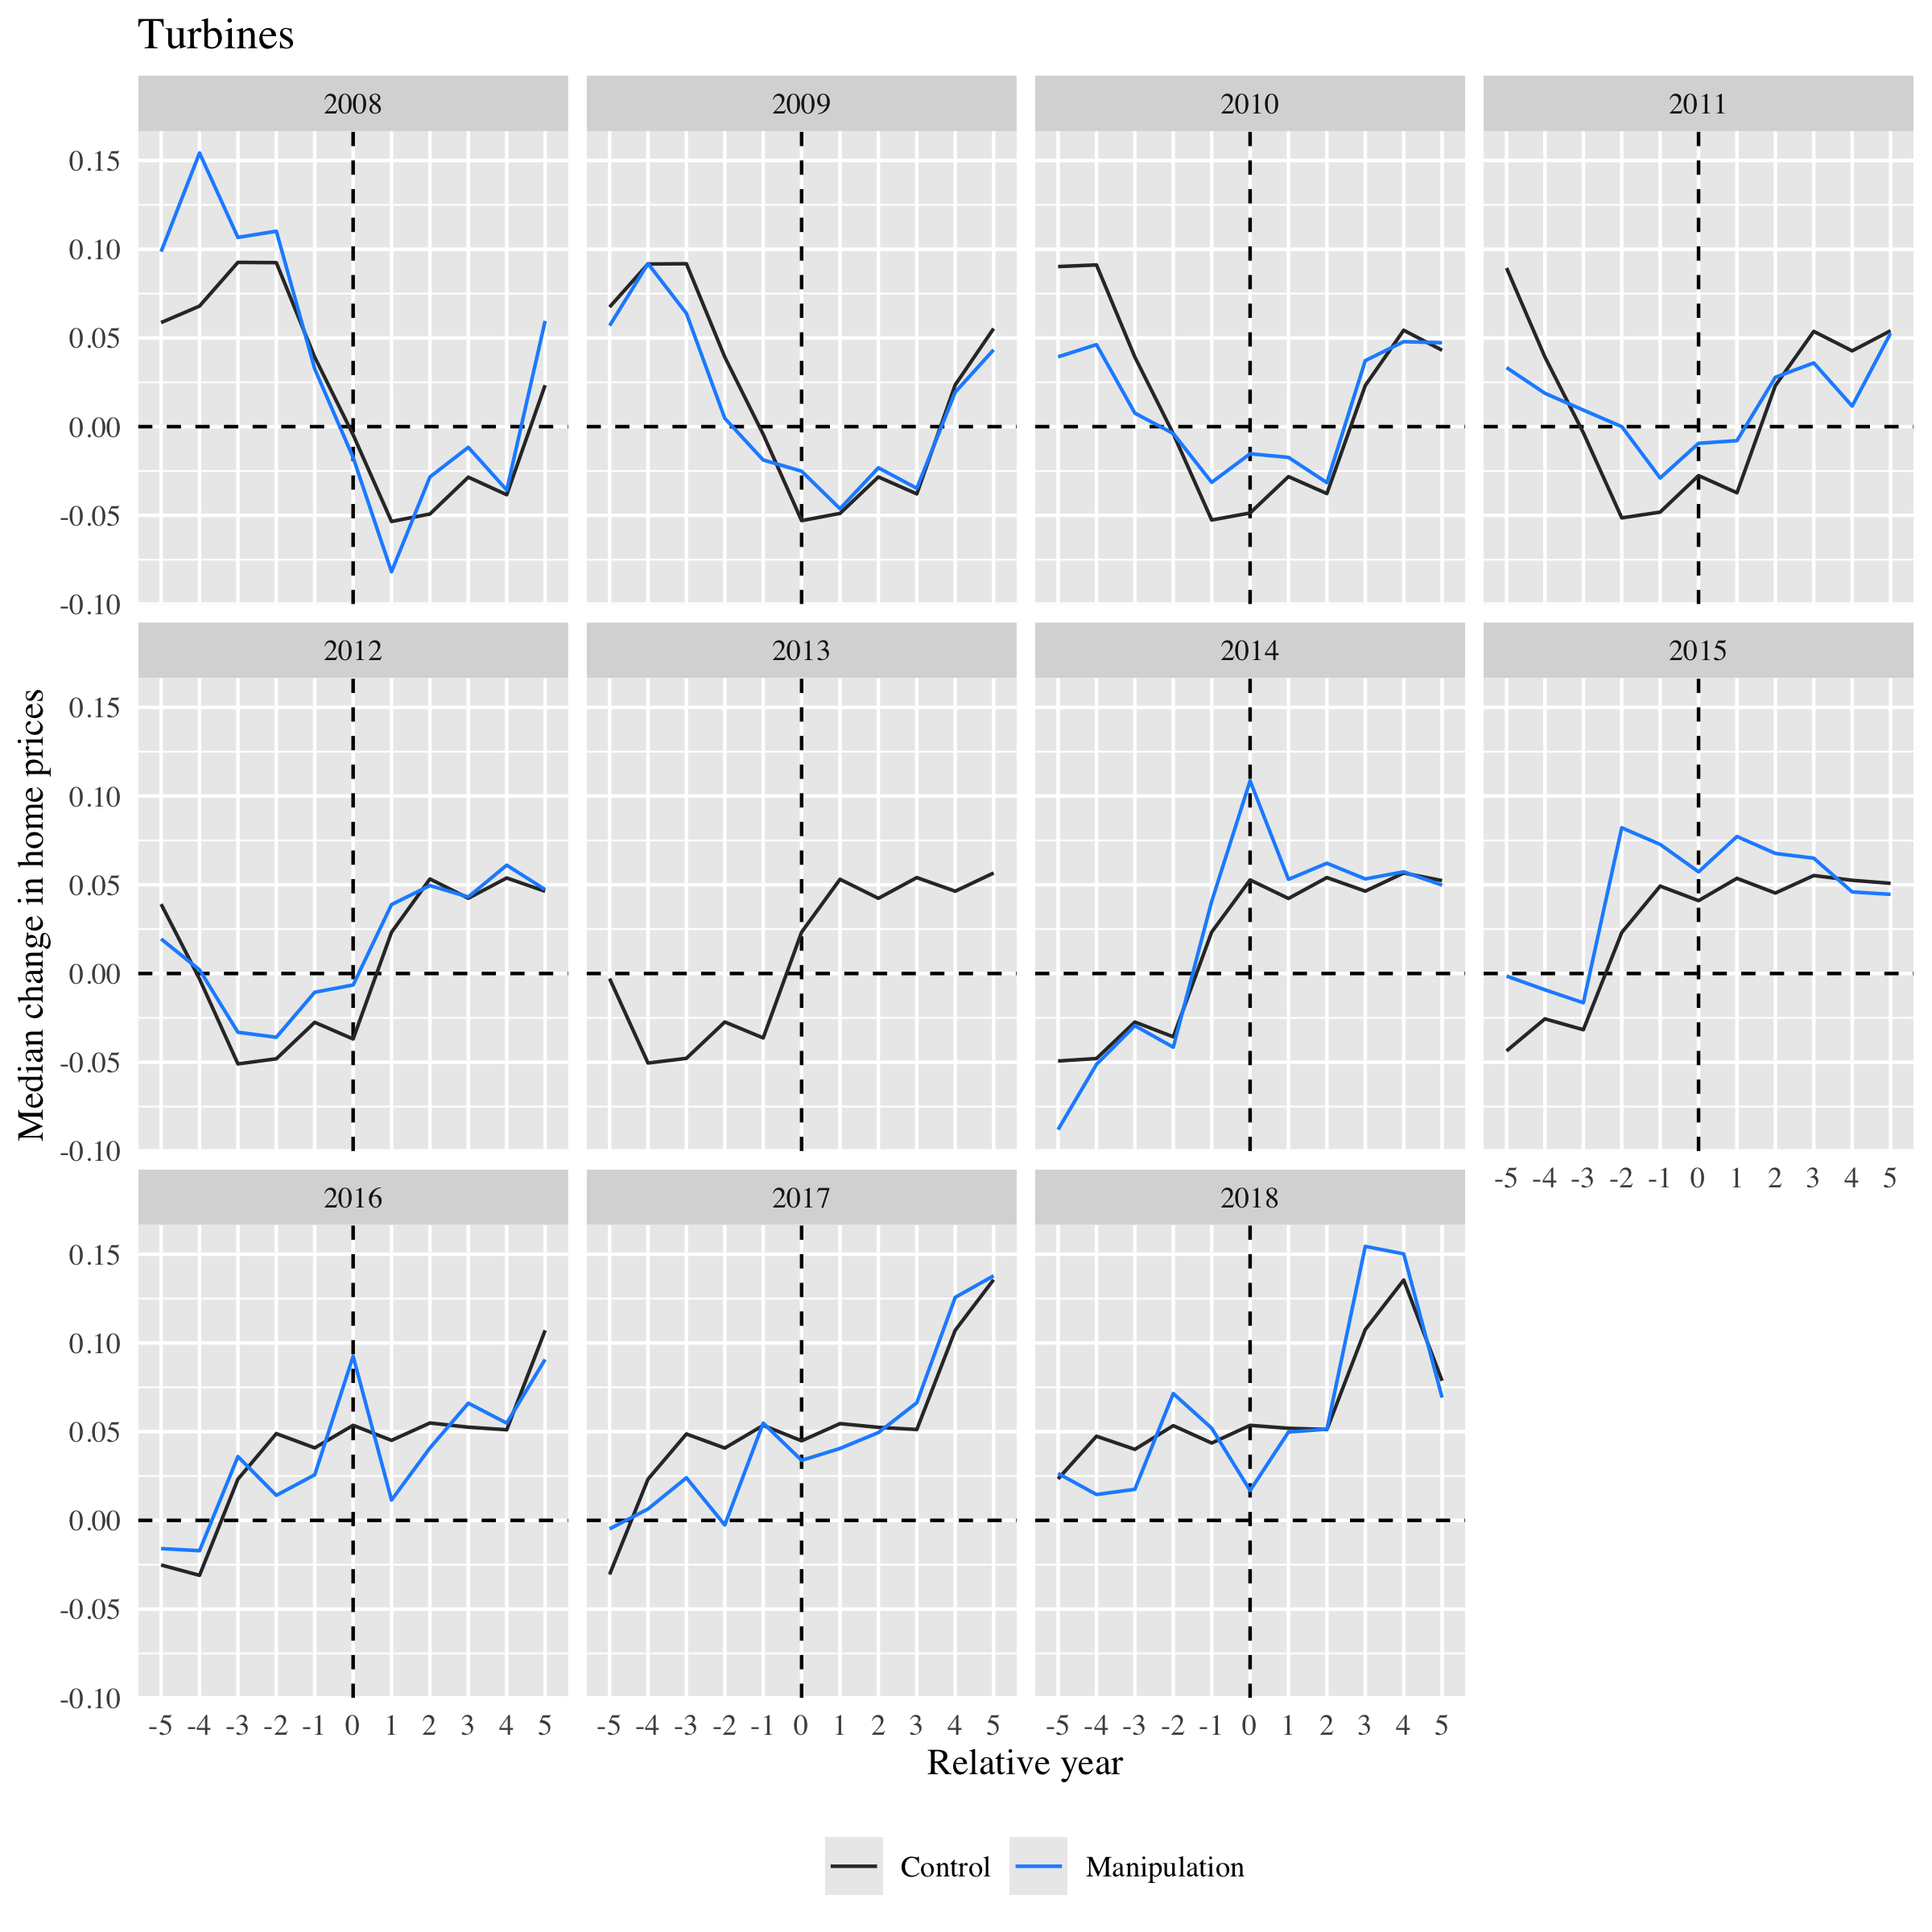
\includegraphics[width=0.9\linewidth]
{study1_turbine_facets.png} 
\caption{Median change in home prices in zip-codes that had wind turbines installed}
\label{study1turbinefacets}
\end{figure}

The other issue with study 1 is small sample size (see figure \ref{study1samplesize}). 
The sample sizes for the manipulation groups pictured here are very small, only a fraction of the size of the control group.
In addition to this problem, while the observations in the manipulation group change in each of the diagrams, the observations in the manipulation group changes completely. 
This means that individual outliers in the control group might be skewing our results.
\begin{figure}[h]
\centering
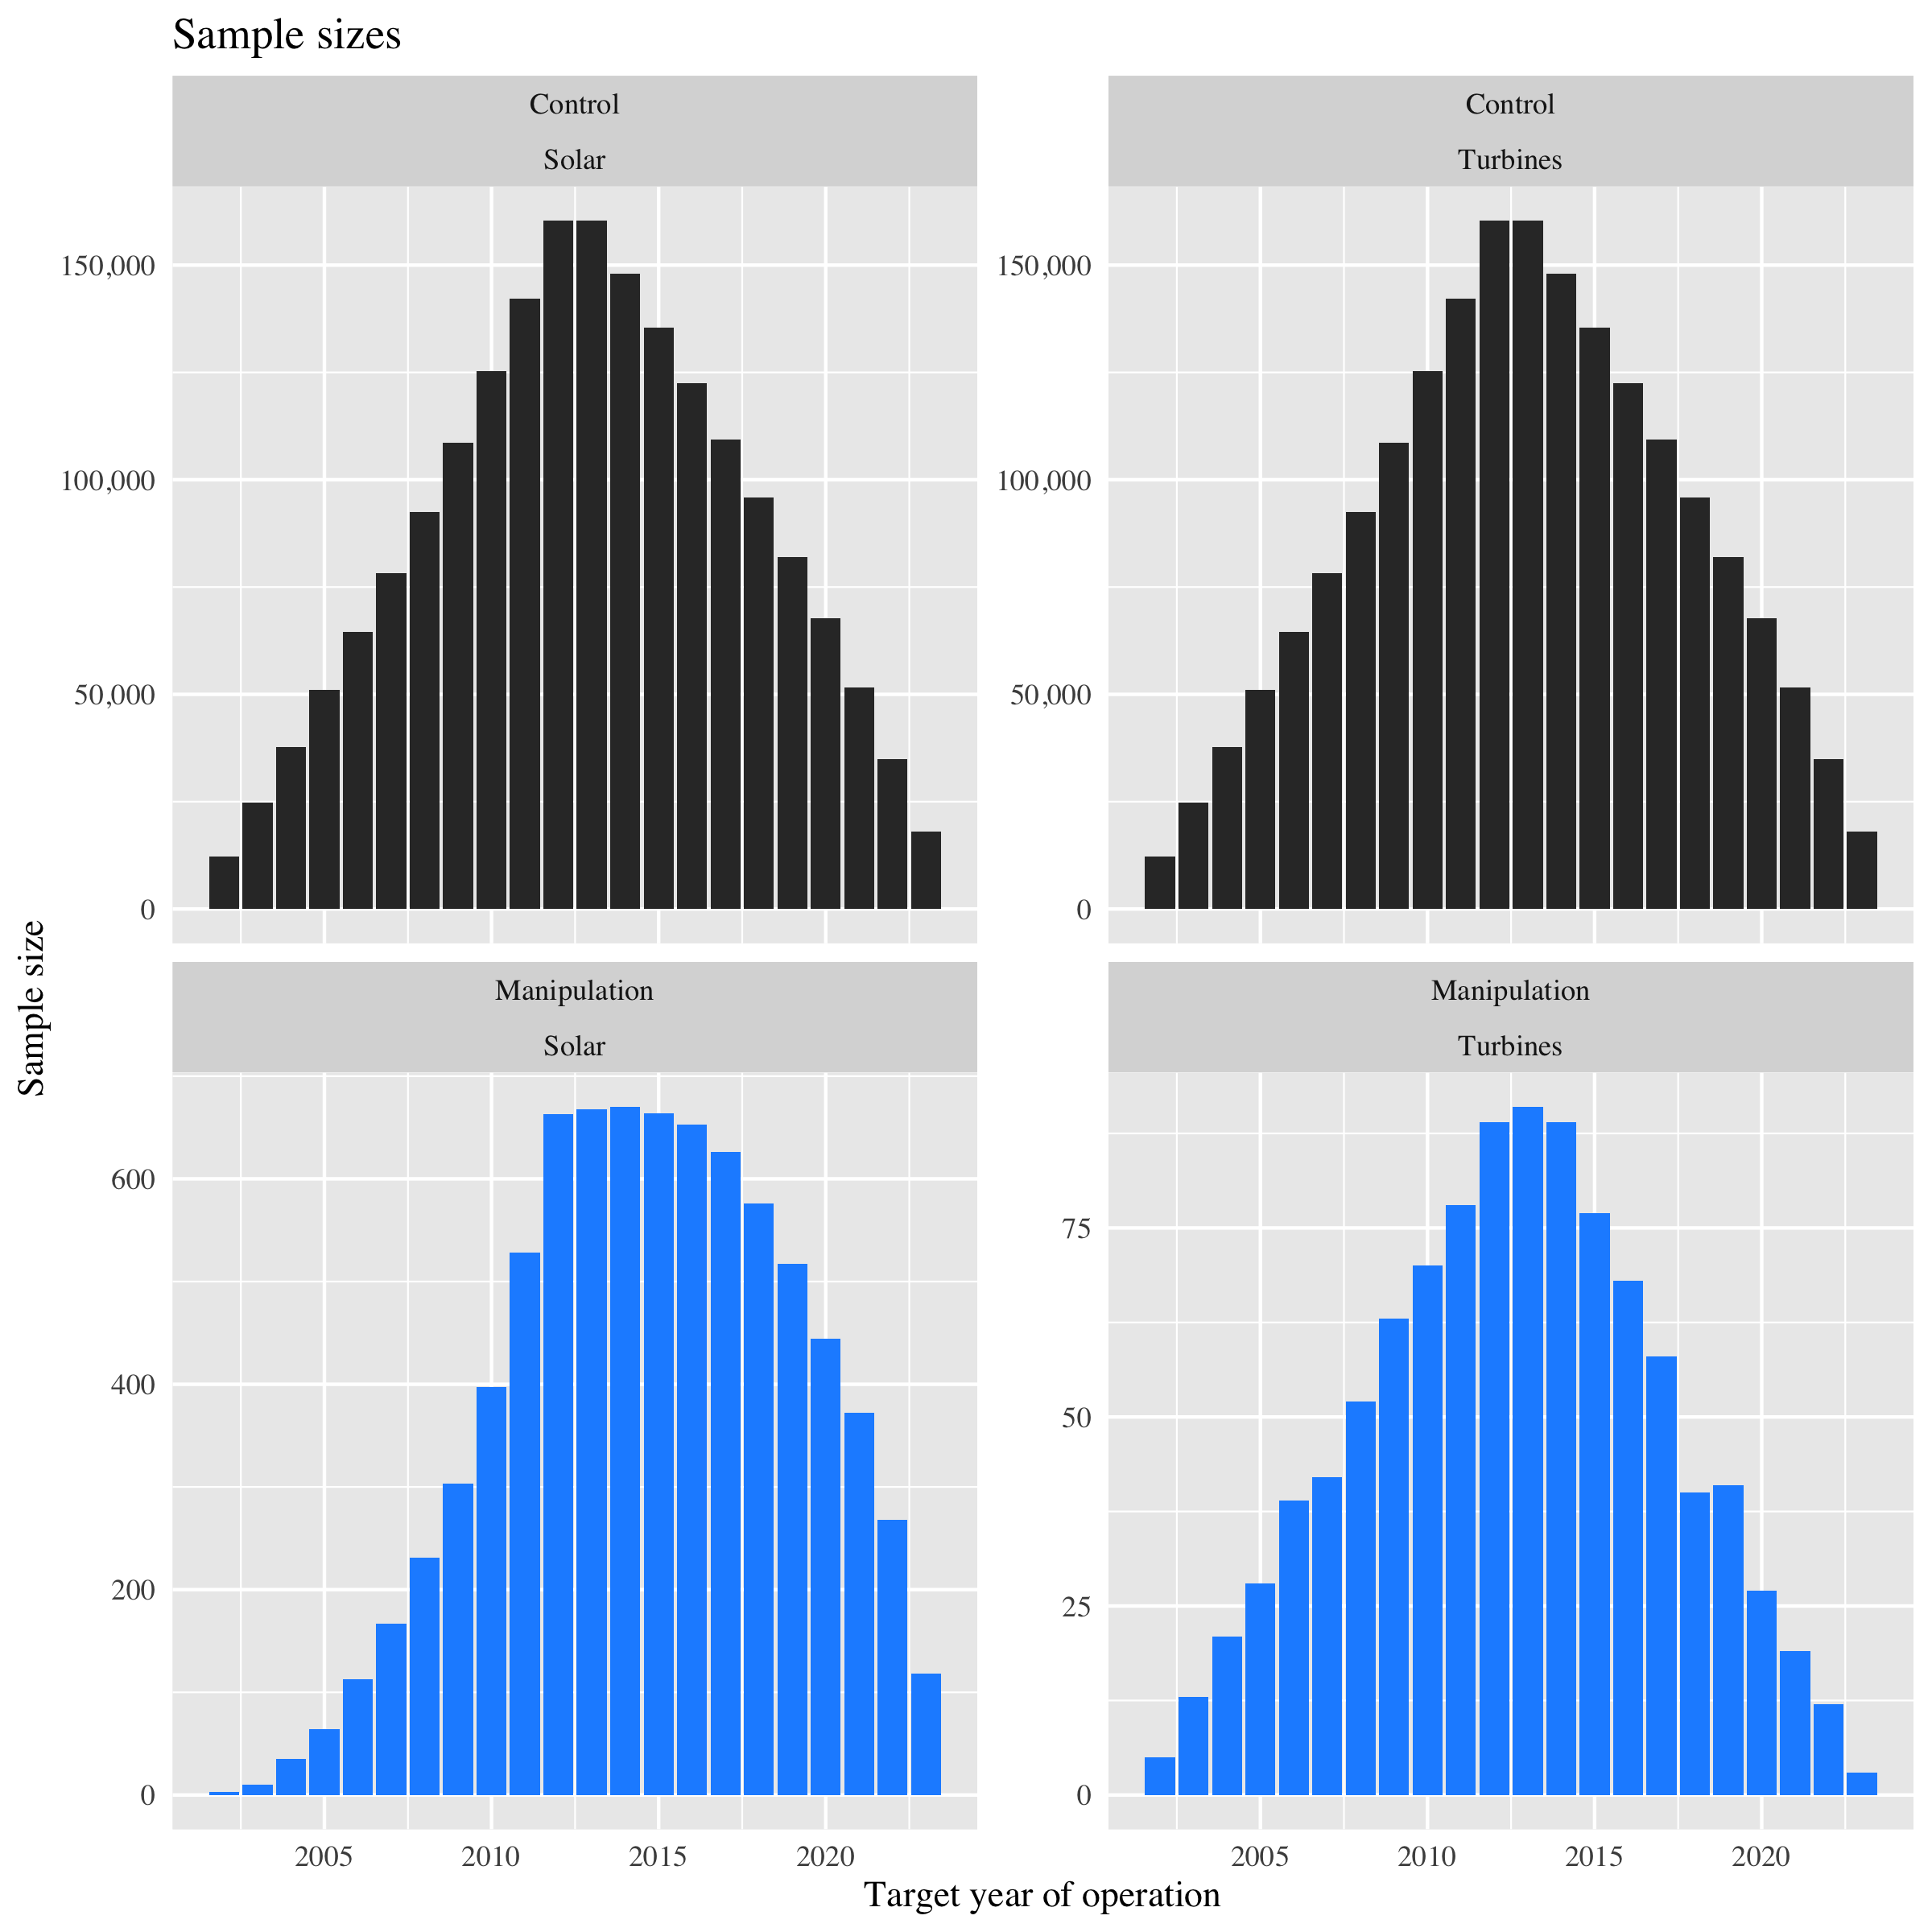
\includegraphics[width=0.9\linewidth]
{study1_sample_size.png} 
\caption{The manipulation groups in study 1 were extremely small}
\label{study1samplesize}
\end{figure}

This brings us to study 2.
Study 2 isn't a classic 'difference-in-difference' two-way fixed-effects study, because it controls for these issues using 1. more fixed-effects and 2. random effects.

\end{document}

Study 2

Study 2 is simply a mixed-effects linear regression model.
The formula for our model looks like this:
change in home price v. last year ~ year + solar_manipulation + turbine_manipulation + (1|zip_code)
Interpretation:
change in home price is the same as it was in study 1: (current home price - last year's home price) / (last year's home price).
Year is the calendar year, represented as an unordered factor. 
Solar manipulation:
if a zip code ever had a solar plant built there, we encode the zip-code each year as one of the following:
Construction: if only one solar plant is built in this zip-code, this is the year of operation. If multiple solar plants are built in this zip-code, this represents the duration between the first plant's year of operation and the last plant's year of operation. Construction indicates that we have faith that during this time period, workers and trucks were around.
-5:-1: Years prior to year of first plant's operation
1:5: Likewise, years after last plant's operation
Censored: any year outside this -5:+5 range in a zip-code that will/has had solar plants

Turbine manipulation:
same encoding as solar manipulation

Note that this model has a few advantages over study 1: we're accounting for general market swings by including year as a fixed-effect, and we can handle zip-codes that have multiple improvements built on them (in study 1, we only included a zip-code as a manipulation if it had either one solar facility or one turbine).

zip-code: here, we model all zip-codes as random intercepts. This compensates for the mean difference in home appreciation in each zip-code

The model is a successful one.
We can compare the model with a null model, in which we omit turbine and solar data:
change in home price v. last year ~ year + (1|zip_code)
Here is the ANOVA comparing the two models. 
As you can see, ...


Here is the intra-class correlation.
The ICC in a multi-level model tests the correlation between the random effects-- here, the zip-codes.
A high ICC would indicate that a lot of the variance that our model is explaining is actually done just by grouping the zip-codes-- this would be an indication that our fixed effects aren't actually that important.
We have a rather low ICC, ...

Here is the full summary as given by R:

And here are the fixed-effects, along with their 95% confidence-intervals.
We can interpret any fixed-effect whose 95% CI doesn't include zero as much more likely to be an observable phenomenon.

Interpretation:






















